% !TEX root=./adl.tex

% -----------------------------------------------------------------------
\begin{frame}{ZeRO: Motivation}

  \emphdef{ZeRO} (Zero Redundancy Optimizer) eliminates memory redundancy in data-parallel training~\cite{rajbhandari2020zero}.

  \vspace{0.5em}
  \begin{columns}
    \begin{column}{0.48\textwidth}
      \textbf{Problem with vanilla DP:}
      \begin{itemize}
        \item Every GPU stores a \emph{full copy} of weights, gradients, and optimizer states
        \item All GPUs compute identical optimizer steps $\Rightarrow$ redundant work and memory
        \item Memory per GPU is $16\Psi$ (mixed-precision Adam) regardless of $N_{\text{DP}}$
      \end{itemize}
    \end{column}
    \begin{column}{0.48\textwidth}
      \textbf{Key insight:}
      \begin{itemize}
        \item Not every GPU \emph{needs} every parameter/gradient/optimizer state at all times
        \item \emph{Partition} these across the DP dimension
        \item Gather on demand via collective communication
        \item Same mathematical result as vanilla DP
      \end{itemize}

      \vspace{0.3em}
      \textbf{PyTorch implementation:}\\
      ZeRO-3 = \emphdef{FSDP} (Fully Sharded Data Parallelism)
    \end{column}
  \end{columns}
\end{frame}

% -----------------------------------------------------------------------
\begin{frame}{Memory Baseline: Mixed-Precision Training with Adam}

  For a model with $\Psi$ parameters using BF16 mixed-precision training:

  \vspace{0.3em}
  \begin{center}
  \begin{tabular}{lll}
    \toprule
    \textbf{Component} & \textbf{Precision} & \textbf{Memory} \\
    \midrule
    Model parameters        & BF16 & $2\Psi$ \\
    Gradients               & BF16 & $2\Psi$ \\
    \midrule
    Master weights (FP32 copy) & FP32 & $4\Psi$ \\
    Adam momentum           & FP32 & $4\Psi$ \\
    Adam variance           & FP32 & $4\Psi$ \\
    \midrule[\heavyrulewidth]
    \textbf{Total}          &      & $\bm{16\Psi}$ \\
    \bottomrule
  \end{tabular}
  \end{center}

  \vspace{0.3em}
  \begin{itemize}\small
    \item \textbf{Optimizer states:} $k\Psi = 12\Psi$ bytes (master weights + momentum + variance)
    \item \textbf{Activations:} not included, depend on batch/seq.\ length, \emph{different} per DP replica
  \end{itemize}

  \vspace{0.3em}
  \begin{center}\small
  \begin{tabular}{rcccc}
    \toprule
    \textbf{Model} & 1B & 7B & 70B & 405B \\
    \midrule
    \textbf{Memory} & 16\,GB & 112\,GB & 1120\,GB & 6480\,GB \\
    \bottomrule
  \end{tabular}
  \end{center}
\end{frame}

% -----------------------------------------------------------------------
% Colors matching the ultra-scale playbook figure
\definecolor{paramcol}{HTML}{4EA5B7}   % teal
\definecolor{gradcol}{HTML}{E889AB}    % pink
\definecolor{optimcol}{HTML}{CEC0FA}   % lavender

\begin{frame}{ZeRO Stages: Memory per GPU}

  \begin{center}
  \begin{tikzpicture}[x=1cm, y=1cm]
    % --- Dimensions ---
    \def\fw{1.6}      % full bar width
    \def\sw{0.22}     % sharded bar width (~1/N_d)
    \def\ph{0.22}     % params bar height
    \def\gh{0.22}     % grads bar height
    \def\oh{0.65}     % optimizer states bar height (~3x)
    \def\colA{2.2}    % GPU_1 column x
    \def\colB{4.8}    % GPU_i column x
    \def\colC{7.4}    % GPU_N column x
    \def\formulaX{9.8} % formula column x
    % Shard offsets within the full-width region (different slice per GPU)
    \def\soA{0}                    % GPU_1: left edge
    \def\soB{0.69}                 % GPU_i: middle
    \def\soC{1.38}                 % GPU_N: right edge (fw - sw)

    % --- Column headers ---
    \node[font=\footnotesize\bfseries] at (\colA+\fw/2, 0.4)
      {GPU$_1$};
    \node[font=\footnotesize\bfseries] at (\colB+\fw/2, 0.4)
      {GPU$_i$};
    \node[font=\footnotesize\bfseries] at (\colC+\fw/2, 0.4)
      {GPU$_{N_d}$};
    \node[font=\footnotesize\bfseries] at (\formulaX, 0.4)
      {Memory};

    % === Helper macro: draw a stacked bar (params, grads, optim) ===
    % Args: x-origin, y-origin (bottom), width
    % Draws bottom-to-top: optimizer states, gradients, parameters

    % ============================================================
    % Row 1: Baseline — all full
    % ============================================================
    \def\ry{-0.3}
    \node[font=\footnotesize\bfseries, anchor=east] at (1.8, \ry-0.55) {Baseline};
    % GPU_1
    \fill[paramcol] (\colA, \ry) rectangle ++(\fw, -\ph);
    \fill[gradcol]  (\colA, \ry-\ph) rectangle ++(\fw, -\gh);
    \fill[optimcol] (\colA, \ry-\ph-\gh) rectangle ++(\fw, -\oh);
    % GPU_i
    \fill[paramcol] (\colB, \ry) rectangle ++(\fw, -\ph);
    \fill[gradcol]  (\colB, \ry-\ph) rectangle ++(\fw, -\gh);
    \fill[optimcol] (\colB, \ry-\ph-\gh) rectangle ++(\fw, -\oh);
    % GPU_N
    \fill[paramcol] (\colC, \ry) rectangle ++(\fw, -\ph);
    \fill[gradcol]  (\colC, \ry-\ph) rectangle ++(\fw, -\gh);
    \fill[optimcol] (\colC, \ry-\ph-\gh) rectangle ++(\fw, -\oh);
    % dots
    \node[font=\footnotesize, gray] at ({(\colA+\fw+\colB)/2}, \ry-0.55) {\dots};
    \node[font=\footnotesize, gray] at ({(\colB+\fw+\colC)/2}, \ry-0.55) {\dots};
    % formula
    \node[font=\footnotesize, anchor=west] at (\formulaX-0.5, \ry-0.55)
      {$2\Psi + 2\Psi + k\Psi$};

    % separator
    \draw[black!40] (1.9, -1.5) -- (\formulaX+0.8, -1.5);

    % ============================================================
    % Row 2: ZeRO-1 — optimizer states sharded
    % ============================================================
    \def\ry{-1.7}
    \node[font=\footnotesize\bfseries, anchor=east] at (1.8, \ry-0.55) {ZeRO-1};
    % GPU_1 — params+grads full, optim shard at left
    \fill[paramcol] (\colA, \ry) rectangle ++(\fw, -\ph);
    \fill[gradcol]  (\colA, \ry-\ph) rectangle ++(\fw, -\gh);
    \fill[optimcol] (\colA+\soA, \ry-\ph-\gh) rectangle ++(\sw, -\oh);
    % GPU_i — optim shard in middle
    \fill[paramcol] (\colB, \ry) rectangle ++(\fw, -\ph);
    \fill[gradcol]  (\colB, \ry-\ph) rectangle ++(\fw, -\gh);
    \fill[optimcol] (\colB+\soB, \ry-\ph-\gh) rectangle ++(\sw, -\oh);
    % GPU_N — optim shard at right
    \fill[paramcol] (\colC, \ry) rectangle ++(\fw, -\ph);
    \fill[gradcol]  (\colC, \ry-\ph) rectangle ++(\fw, -\gh);
    \fill[optimcol] (\colC+\soC, \ry-\ph-\gh) rectangle ++(\sw, -\oh);
    % dots
    \node[font=\footnotesize, gray] at ({(\colA+\fw+\colB)/2}, \ry-0.55) {\dots};
    \node[font=\footnotesize, gray] at ({(\colB+\fw+\colC)/2}, \ry-0.55) {\dots};
    % formula
    \node[font=\footnotesize, anchor=west] at (\formulaX-0.5, \ry-0.55)
      {$2\Psi + 2\Psi + \dfrac{k\Psi}{N_d}$};

    % separator
    \draw[black!40] (1.9, -2.9) -- (\formulaX+0.8, -2.9);

    % ============================================================
    % Row 3: ZeRO-2 — optim + grads sharded
    % ============================================================
    \def\ry{-3.1}
    \node[font=\footnotesize\bfseries, anchor=east] at (1.8, \ry-0.55) {ZeRO-2};
    % GPU_1 — params full, grads+optim shard at left
    \fill[paramcol] (\colA, \ry) rectangle ++(\fw, -\ph);
    \fill[gradcol]  (\colA+\soA, \ry-\ph) rectangle ++(\sw, -\gh);
    \fill[optimcol] (\colA+\soA, \ry-\ph-\gh) rectangle ++(\sw, -\oh);
    % GPU_i — grads+optim shard in middle
    \fill[paramcol] (\colB, \ry) rectangle ++(\fw, -\ph);
    \fill[gradcol]  (\colB+\soB, \ry-\ph) rectangle ++(\sw, -\gh);
    \fill[optimcol] (\colB+\soB, \ry-\ph-\gh) rectangle ++(\sw, -\oh);
    % GPU_N — grads+optim shard at right
    \fill[paramcol] (\colC, \ry) rectangle ++(\fw, -\ph);
    \fill[gradcol]  (\colC+\soC, \ry-\ph) rectangle ++(\sw, -\gh);
    \fill[optimcol] (\colC+\soC, \ry-\ph-\gh) rectangle ++(\sw, -\oh);
    % dots
    \node[font=\footnotesize, gray] at ({(\colA+\fw+\colB)/2}, \ry-0.55) {\dots};
    \node[font=\footnotesize, gray] at ({(\colB+\fw+\colC)/2}, \ry-0.55) {\dots};
    % formula
    \node[font=\footnotesize, anchor=west] at (\formulaX-0.5, \ry-0.55)
      {$2\Psi + \dfrac{(2+k)\Psi}{N_d}$};

    % separator
    \draw[black!40] (1.9, -4.3) -- (\formulaX+0.8, -4.3);

    % ============================================================
    % Row 4: ZeRO-3 — everything sharded
    % ============================================================
    \def\ry{-4.5}
    \node[font=\footnotesize\bfseries, anchor=east] at (1.8, \ry-0.55) {ZeRO-3};
    % GPU_1 — all sharded at left
    \fill[paramcol] (\colA+\soA, \ry) rectangle ++(\sw, -\ph);
    \fill[gradcol]  (\colA+\soA, \ry-\ph) rectangle ++(\sw, -\gh);
    \fill[optimcol] (\colA+\soA, \ry-\ph-\gh) rectangle ++(\sw, -\oh);
    % GPU_i — all sharded in middle
    \fill[paramcol] (\colB+\soB, \ry) rectangle ++(\sw, -\ph);
    \fill[gradcol]  (\colB+\soB, \ry-\ph) rectangle ++(\sw, -\gh);
    \fill[optimcol] (\colB+\soB, \ry-\ph-\gh) rectangle ++(\sw, -\oh);
    % GPU_N — all sharded at right
    \fill[paramcol] (\colC+\soC, \ry) rectangle ++(\sw, -\ph);
    \fill[gradcol]  (\colC+\soC, \ry-\ph) rectangle ++(\sw, -\gh);
    \fill[optimcol] (\colC+\soC, \ry-\ph-\gh) rectangle ++(\sw, -\oh);
    % dots
    \node[font=\footnotesize, gray] at ({(\colA+\fw+\colB)/2}, \ry-0.55) {\dots};
    \node[font=\footnotesize, gray] at ({(\colB+\fw+\colC)/2}, \ry-0.55) {\dots};
    % formula
    \node[font=\footnotesize, anchor=west] at (\formulaX-0.5, \ry-0.55)
      {$\dfrac{(2+2+k)\Psi}{N_d}$};

    % ============================================================
    % Legend (bottom)
    % ============================================================
    \fill[paramcol] (\colA, -5.85) rectangle ++(1.6, -0.35);
    \node[font=\scriptsize, white] at (\colA+0.8, -6.025) {Parameters};
    \fill[gradcol]  (\colB, -5.85) rectangle ++(1.6, -0.35);
    \node[font=\scriptsize, white] at (\colB+0.8, -6.025) {Gradients};
    \fill[optimcol] (\colC, -5.85) rectangle ++(1.6, -0.35);
    \node[font=\scriptsize] at (\colC+0.8, -6.025) {Optimizer States};

    % Variable definitions
    \node[font=\tiny, anchor=west, align=left] at (\formulaX-0.5, -6.1)
      {$\Psi$: \#params, $k\!=\!12$ (Adam)\\$N_d$: DP degree};

  \end{tikzpicture}
  \end{center}
\end{frame}

% -----------------------------------------------------------------------
\begin{frame}{ZeRO-1: Illustrated ($N_d = 3$)}

  % Shows model as 6 layers. Params \& grads fully replicated on each GPU.
  % Optimizer states partitioned: each GPU owns 2 layers' worth.
  \begin{center}
  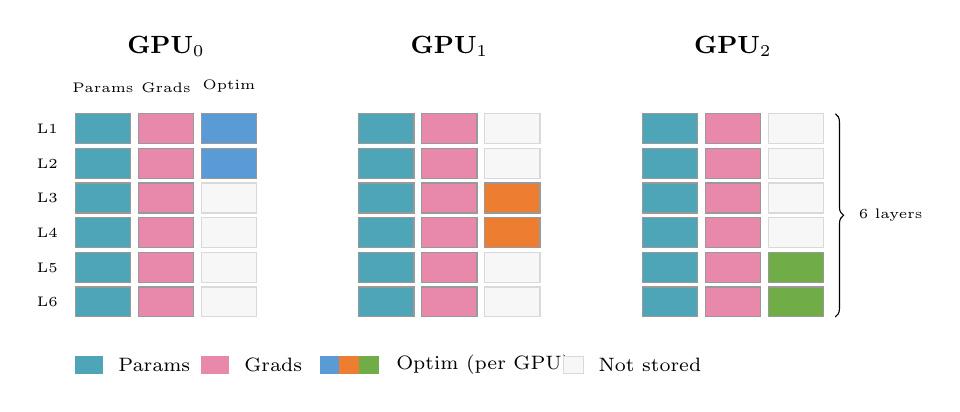
\begin{tikzpicture}[x=1cm, y=1cm]
    % --- colors for GPU ownership ---
    \definecolor{g0}{HTML}{5B9BD5}   % blue
    \definecolor{g1}{HTML}{ED7D31}   % orange
    \definecolor{g2}{HTML}{70AD47}   % green

    % --- dimensions ---
    \def\lh{0.38}     % layer block height
    \def\lg{0.06}     % gap between layers
    \def\lw{0.7}      % column width per section
    \def\sg{0.1}      % gap between sections (params/grads/optim)
    \def\gx{3.6}      % horizontal gap between GPUs
    \def\NL{6}        % number of layers

    % --- derived ---
    % total stack height = 6*(lh+lg) - lg = 6*0.44 - 0.06 = 2.58

    % =============================================
    % GPU columns
    % =============================================
    \foreach \g in {0,1,2} {
      \pgfmathsetmacro{\bx}{\g*\gx}

      % GPU label
      \node[font=\small\bfseries] at ({\bx+1.5*\lw+\sg}, 0.85) {GPU$_\g$};

      % Section headers (horizontal, only for first GPU to avoid clutter)
      \ifnum\g=0
        \node[font=\tiny, anchor=south] at ({\bx+\lw/2}, 0.15) {Params};
        \node[font=\tiny, anchor=south] at ({\bx+\lw+\sg+\lw/2}, 0.15) {Grads};
        \node[font=\tiny, anchor=south] at ({\bx+2*\lw+2*\sg+\lw/2}, 0.15) {Optim};
      \fi

      % Draw 6 layers for each section
      \foreach \l in {0,1,2,3,4,5} {
        \pgfmathsetmacro{\ly}{-\l*(\lh+\lg)}

        % Params column — all layers filled (replicated)
        \fill[paramcol] (\bx, \ly) rectangle ++(\lw, -\lh);
        \draw[black!40] (\bx, \ly) rectangle ++(\lw, -\lh);

        % Grads column — all layers filled (replicated)
        \fill[gradcol] ({\bx+\lw+\sg}, \ly) rectangle ++(\lw, -\lh);
        \draw[black!40] ({\bx+\lw+\sg}, \ly) rectangle ++(\lw, -\lh);

        % Optim column — only this GPU's 2 layers filled
        \pgfmathsetmacro{\ownstart}{int(\g*2)}
        \pgfmathsetmacro{\ownend}{int(\g*2+1)}
        \pgfmathtruncatemacro{\isOwned}{(\l>=\ownstart && \l<=\ownend) ? 1 : 0}
        \ifnum\isOwned=1
          % Filled with GPU's color
          \pgfmathtruncatemacro{\gi}{\g}
          \fill[g\gi] ({\bx+2*\lw+2*\sg}, \ly) rectangle ++(\lw, -\lh);
          \draw[black!40] ({\bx+2*\lw+2*\sg}, \ly) rectangle ++(\lw, -\lh);
        \else
          % Empty (not stored)
          \draw[black!15, fill=black!3] ({\bx+2*\lw+2*\sg}, \ly) rectangle ++(\lw, -\lh);
        \fi
      }

      % Layer labels (only for first GPU)
      \ifnum\g=0
        \foreach \l in {0,1,2,3,4,5} {
          \pgfmathsetmacro{\ly}{-\l*(\lh+\lg)}
          \pgfmathtruncatemacro{\ll}{\l+1}
          \node[font=\tiny, anchor=east] at (-0.1, {\ly-\lh/2}) {L\ll};
        }
      \fi
    }

    % =============================================
    % Brace + memory labels
    % =============================================
    % Brace on the right side of GPU 2's optim column
    \pgfmathsetmacro{\bracex}{2*\gx+3*\lw+2*\sg+0.15}
    \draw[decorate, decoration={brace, amplitude=3pt}]
      (\bracex, 0) -- (\bracex, {-5*(\lh+\lg)-\lh})
      node[midway, font=\tiny, anchor=west, xshift=5pt, align=left] {6 layers};

    % =============================================
    % Legend
    % =============================================
    \def\ly{-3.3}
    \fill[paramcol] (0, \ly) rectangle ++(0.35, 0.22);
    \node[font=\scriptsize, anchor=west] at (0.42, {\ly+0.11}) {Params};
    \fill[gradcol] (1.6, \ly) rectangle ++(0.35, 0.22);
    \node[font=\scriptsize, anchor=west] at (2.02, {\ly+0.11}) {Grads};
    \fill[g0] (3.1, \ly) rectangle ++(0.25, 0.22);
    \fill[g1] (3.35, \ly) rectangle ++(0.25, 0.22);
    \fill[g2] (3.6, \ly) rectangle ++(0.25, 0.22);
    \node[font=\scriptsize, anchor=west] at (3.95, {\ly+0.11}) {Optim (per GPU)};
    \fill[black!3] (6.2, \ly) rectangle ++(0.25, 0.22);
    \draw[black!15] (6.2, \ly) rectangle ++(0.25, 0.22);
    \node[font=\scriptsize, anchor=west] at (6.52, {\ly+0.11}) {Not stored};

  \end{tikzpicture}
  \end{center}

  {\small\textbf{Algorithm:}}
  \begin{enumerate}\small\setlength{\itemsep}{0pt}\setlength{\parskip}{0pt}
    \item Fwd+Bwd as in vanilla DP $\to$ full grads on each GPU
    \item \textsc{ReduceScatter} grads: each GPU receives its $\frac{1}{N_d}$ slice (summed)
    \item Each GPU runs optimizer on its slice only
    \item \textsc{AllGather} updated params to reconstruct full model
  \end{enumerate}
  {\small\textbf{Memory:} $4\Psi + \tfrac{12\Psi}{N_d}$ per GPU.
  \quad \textbf{Comm:} same as DP AllReduce ($2\Psi$).}
\end{frame}

% -----------------------------------------------------------------------
\begin{frame}{ZeRO-2: Illustrated ($N_d = 3$)}

  % Shows model as 6 layers. Params replicated, grads + optim partitioned.
  \begin{center}
  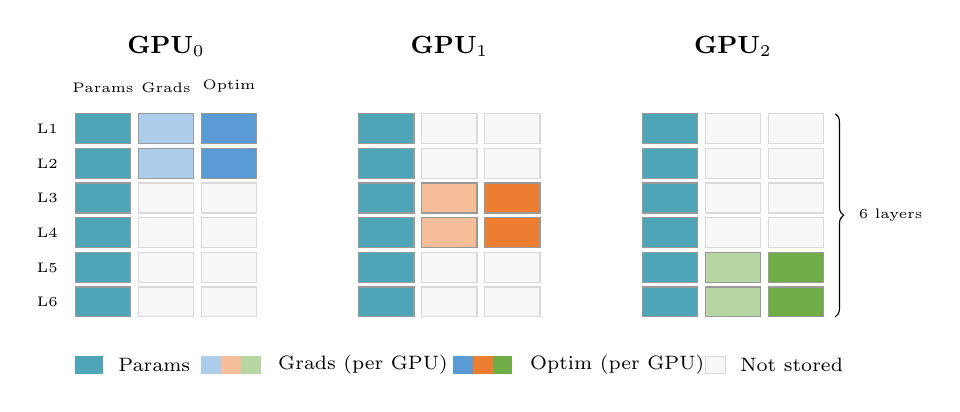
\begin{tikzpicture}[x=1cm, y=1cm]
    % --- colors for GPU ownership ---
    \definecolor{g0}{HTML}{5B9BD5}   % blue
    \definecolor{g1}{HTML}{ED7D31}   % orange
    \definecolor{g2}{HTML}{70AD47}   % green

    % --- dimensions ---
    \def\lh{0.38}     % layer block height
    \def\lg{0.06}     % gap between layers
    \def\lw{0.7}      % column width per section
    \def\sg{0.1}      % gap between sections
    \def\gx{3.6}      % horizontal gap between GPUs

    % =============================================
    % GPU columns
    % =============================================
    \foreach \g in {0,1,2} {
      \pgfmathsetmacro{\bx}{\g*\gx}

      % GPU label
      \node[font=\small\bfseries] at ({\bx+1.5*\lw+\sg}, 0.85) {GPU$_\g$};

      % Section headers (only for first GPU)
      \ifnum\g=0
        \node[font=\tiny, anchor=south] at ({\bx+\lw/2}, 0.15) {Params};
        \node[font=\tiny, anchor=south] at ({\bx+\lw+\sg+\lw/2}, 0.15) {Grads};
        \node[font=\tiny, anchor=south] at ({\bx+2*\lw+2*\sg+\lw/2}, 0.15) {Optim};
      \fi

      % Draw 6 layers for each section
      \foreach \l in {0,1,2,3,4,5} {
        \pgfmathsetmacro{\ly}{-\l*(\lh+\lg)}

        % Params column — all layers filled (replicated)
        \fill[paramcol] (\bx, \ly) rectangle ++(\lw, -\lh);
        \draw[black!40] (\bx, \ly) rectangle ++(\lw, -\lh);

        % Grads column — only this GPU's 2 layers filled (partitioned)
        \pgfmathsetmacro{\ownstart}{int(\g*2)}
        \pgfmathsetmacro{\ownend}{int(\g*2+1)}
        \pgfmathtruncatemacro{\isOwned}{(\l>=\ownstart && \l<=\ownend) ? 1 : 0}
        \ifnum\isOwned=1
          \pgfmathtruncatemacro{\gi}{\g}
          \fill[g\gi!50] ({\bx+\lw+\sg}, \ly) rectangle ++(\lw, -\lh);
          \draw[black!40] ({\bx+\lw+\sg}, \ly) rectangle ++(\lw, -\lh);
        \else
          \draw[black!15, fill=black!3] ({\bx+\lw+\sg}, \ly) rectangle ++(\lw, -\lh);
        \fi

        % Optim column — only this GPU's 2 layers filled (partitioned)
        \ifnum\isOwned=1
          \fill[g\gi] ({\bx+2*\lw+2*\sg}, \ly) rectangle ++(\lw, -\lh);
          \draw[black!40] ({\bx+2*\lw+2*\sg}, \ly) rectangle ++(\lw, -\lh);
        \else
          \draw[black!15, fill=black!3] ({\bx+2*\lw+2*\sg}, \ly) rectangle ++(\lw, -\lh);
        \fi
      }

      % Layer labels (only for first GPU)
      \ifnum\g=0
        \foreach \l in {0,1,2,3,4,5} {
          \pgfmathsetmacro{\ly}{-\l*(\lh+\lg)}
          \pgfmathtruncatemacro{\ll}{\l+1}
          \node[font=\tiny, anchor=east] at (-0.1, {\ly-\lh/2}) {L\ll};
        }
      \fi
    }

    % Brace on the right side of GPU 2
    \pgfmathsetmacro{\bracex}{2*\gx+3*\lw+2*\sg+0.15}
    \draw[decorate, decoration={brace, amplitude=3pt}]
      (\bracex, 0) -- (\bracex, {-5*(\lh+\lg)-\lh})
      node[midway, font=\tiny, anchor=west, xshift=5pt, align=left] {6 layers};

    % Legend
    \def\ly{-3.3}
    \fill[paramcol] (0, \ly) rectangle ++(0.35, 0.22);
    \node[font=\scriptsize, anchor=west] at (0.42, {\ly+0.11}) {Params};
    \fill[g0!50] (1.6, \ly) rectangle ++(0.25, 0.22);
    \fill[g1!50] (1.85, \ly) rectangle ++(0.25, 0.22);
    \fill[g2!50] (2.1, \ly) rectangle ++(0.25, 0.22);
    \node[font=\scriptsize, anchor=west] at (2.45, {\ly+0.11}) {Grads (per GPU)};
    \fill[g0] (4.8, \ly) rectangle ++(0.25, 0.22);
    \fill[g1] (5.05, \ly) rectangle ++(0.25, 0.22);
    \fill[g2] (5.3, \ly) rectangle ++(0.25, 0.22);
    \node[font=\scriptsize, anchor=west] at (5.65, {\ly+0.11}) {Optim (per GPU)};
    \fill[black!3] (8.0, \ly) rectangle ++(0.25, 0.22);
    \draw[black!15] (8.0, \ly) rectangle ++(0.25, 0.22);
    \node[font=\scriptsize, anchor=west] at (8.32, {\ly+0.11}) {Not stored};

  \end{tikzpicture}
  \end{center}

  {\small\textbf{Algorithm:}}
  \begin{enumerate}\small\setlength{\itemsep}{0pt}\setlength{\parskip}{0pt}
    \item Fwd+Bwd: \textsc{ReduceScatter} grads \emph{during} backward $\to$ each GPU keeps only its $\frac{1}{N_d}$ slice
    \item Each GPU runs optimizer on its slice only
    \item \textsc{AllGather} updated params to reconstruct full model
  \end{enumerate}
  {\small\textbf{Memory:} $2\Psi + \tfrac{(2+12)\Psi}{N_d}$ per GPU.
  \quad \textbf{Comm:} same as ZeRO-1 ($2\Psi$), strictly better, no overhead.}
\end{frame}

% -----------------------------------------------------------------------
\begin{frame}{ZeRO-3 / FSDP: Illustrated ($N_d = 3$)}

  % Shows model as 6 layers. Everything partitioned.
  \begin{center}
  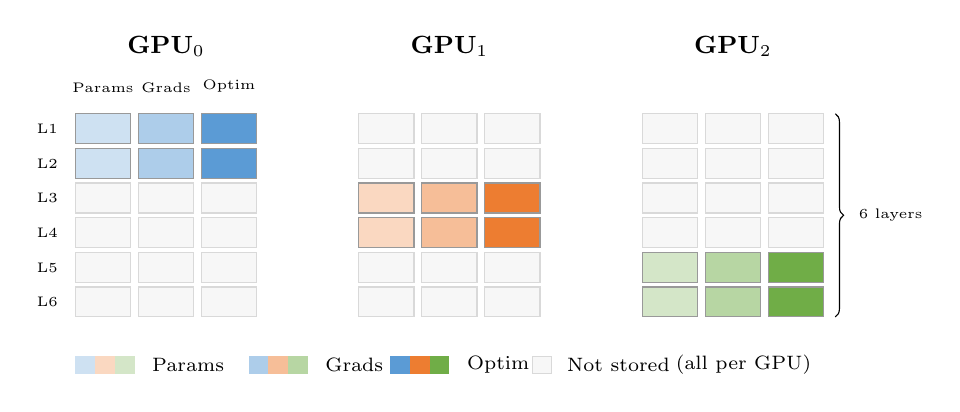
\begin{tikzpicture}[x=1cm, y=1cm]
    % --- colors for GPU ownership ---
    \definecolor{g0}{HTML}{5B9BD5}   % blue
    \definecolor{g1}{HTML}{ED7D31}   % orange
    \definecolor{g2}{HTML}{70AD47}   % green

    % --- dimensions ---
    \def\lh{0.38}     % layer block height
    \def\lg{0.06}     % gap between layers
    \def\lw{0.7}      % column width per section
    \def\sg{0.1}      % gap between sections
    \def\gx{3.6}      % horizontal gap between GPUs

    % =============================================
    % GPU columns
    % =============================================
    \foreach \g in {0,1,2} {
      \pgfmathsetmacro{\bx}{\g*\gx}

      % GPU label
      \node[font=\small\bfseries] at ({\bx+1.5*\lw+\sg}, 0.85) {GPU$_\g$};

      % Section headers (only for first GPU)
      \ifnum\g=0
        \node[font=\tiny, anchor=south] at ({\bx+\lw/2}, 0.15) {Params};
        \node[font=\tiny, anchor=south] at ({\bx+\lw+\sg+\lw/2}, 0.15) {Grads};
        \node[font=\tiny, anchor=south] at ({\bx+2*\lw+2*\sg+\lw/2}, 0.15) {Optim};
      \fi

      % Draw 6 layers for each section
      \foreach \l in {0,1,2,3,4,5} {
        \pgfmathsetmacro{\ly}{-\l*(\lh+\lg)}
        \pgfmathsetmacro{\ownstart}{int(\g*2)}
        \pgfmathsetmacro{\ownend}{int(\g*2+1)}
        \pgfmathtruncatemacro{\isOwned}{(\l>=\ownstart && \l<=\ownend) ? 1 : 0}
        \pgfmathtruncatemacro{\gi}{\g}

        % Params column — partitioned
        \ifnum\isOwned=1
          \fill[g\gi!30] (\bx, \ly) rectangle ++(\lw, -\lh);
          \draw[black!40] (\bx, \ly) rectangle ++(\lw, -\lh);
        \else
          \draw[black!15, fill=black!3] (\bx, \ly) rectangle ++(\lw, -\lh);
        \fi

        % Grads column — partitioned
        \ifnum\isOwned=1
          \fill[g\gi!50] ({\bx+\lw+\sg}, \ly) rectangle ++(\lw, -\lh);
          \draw[black!40] ({\bx+\lw+\sg}, \ly) rectangle ++(\lw, -\lh);
        \else
          \draw[black!15, fill=black!3] ({\bx+\lw+\sg}, \ly) rectangle ++(\lw, -\lh);
        \fi

        % Optim column — partitioned
        \ifnum\isOwned=1
          \fill[g\gi] ({\bx+2*\lw+2*\sg}, \ly) rectangle ++(\lw, -\lh);
          \draw[black!40] ({\bx+2*\lw+2*\sg}, \ly) rectangle ++(\lw, -\lh);
        \else
          \draw[black!15, fill=black!3] ({\bx+2*\lw+2*\sg}, \ly) rectangle ++(\lw, -\lh);
        \fi
      }

      % Layer labels (only for first GPU)
      \ifnum\g=0
        \foreach \l in {0,1,2,3,4,5} {
          \pgfmathsetmacro{\ly}{-\l*(\lh+\lg)}
          \pgfmathtruncatemacro{\ll}{\l+1}
          \node[font=\tiny, anchor=east] at (-0.1, {\ly-\lh/2}) {L\ll};
        }
      \fi
    }

    % Brace on the right side of GPU 2
    \pgfmathsetmacro{\bracex}{2*\gx+3*\lw+2*\sg+0.15}
    \draw[decorate, decoration={brace, amplitude=3pt}]
      (\bracex, 0) -- (\bracex, {-5*(\lh+\lg)-\lh})
      node[midway, font=\tiny, anchor=west, xshift=5pt, align=left] {6 layers};

    % Legend
    \def\ly{-3.3}
    \fill[g0!30] (0, \ly) rectangle ++(0.25, 0.22);
    \fill[g1!30] (0.25, \ly) rectangle ++(0.25, 0.22);
    \fill[g2!30] (0.5, \ly) rectangle ++(0.25, 0.22);
    \node[font=\scriptsize, anchor=west] at (0.85, {\ly+0.11}) {Params};
    \fill[g0!50] (2.2, \ly) rectangle ++(0.25, 0.22);
    \fill[g1!50] (2.45, \ly) rectangle ++(0.25, 0.22);
    \fill[g2!50] (2.7, \ly) rectangle ++(0.25, 0.22);
    \node[font=\scriptsize, anchor=west] at (3.05, {\ly+0.11}) {Grads};
    \fill[g0] (4.0, \ly) rectangle ++(0.25, 0.22);
    \fill[g1] (4.25, \ly) rectangle ++(0.25, 0.22);
    \fill[g2] (4.5, \ly) rectangle ++(0.25, 0.22);
    \node[font=\scriptsize, anchor=west] at (4.85, {\ly+0.11}) {Optim};
    \fill[black!3] (5.8, \ly) rectangle ++(0.25, 0.22);
    \draw[black!15] (5.8, \ly) rectangle ++(0.25, 0.22);
    \node[font=\scriptsize, anchor=west] at (6.12, {\ly+0.11}) {Not stored};
    \node[font=\scriptsize, anchor=west] at (7.5, {\ly+0.11}) {(all per GPU)};

  \end{tikzpicture}
  \end{center}

  {\small\textbf{Key insight:} each layer's params are only needed \emph{during} its fwd/bwd computation.
  So params can be partitioned and gathered \emph{on demand} per layer, then discarded.}

  {\small\textbf{Algorithm:}}
  \begin{enumerate}\small\setlength{\itemsep}{0pt}\setlength{\parskip}{0pt}
    \item \textbf{Fwd:} for each layer $\ell$: \textsc{AllGather} full params from all GPUs $\to$ compute $\to$ \emph{discard} non-local params
    \item \textbf{Bwd:} for each layer $\ell$ (reverse): \textsc{AllGather} params again $\to$ compute grads $\to$ \textsc{ReduceScatter} grads $\to$ discard
    \item Each GPU runs optimizer on its $\frac{1}{N_d}$ slice only
  \end{enumerate}
  {\small\textbf{Memory:} $\tfrac{16\Psi}{N_d}$ per GPU.
  \quad \textbf{Comm:} $3\Psi$ (extra \textsc{AllGather} in fwd).
  \quad PyTorch: \textbf{FSDP}.}
\end{frame}

% -----------------------------------------------------------------------
\begin{frame}{Communication Volume Comparison}

  \begin{center}
  \renewcommand{\arraystretch}{1.3}
  \begin{tabular}{lccl}
    \toprule
    \textbf{Method} & \textbf{Comm.\ Volume} & \textbf{Operations} & \textbf{Memory} \\
    \midrule
    Vanilla DP & $2\Psi$ & AllReduce & $16\Psi$ \\
    ZeRO-1 & $2\Psi$ & RS + AG & $4\Psi + \frac{12\Psi}{N_d}$ \\
    ZeRO-2 & $2\Psi$ & RS + AG & $2\Psi + \frac{14\Psi}{N_d}$ \\
    ZeRO-3 & $3\Psi$ & $2\times$AG + RS & $\frac{16\Psi}{N_d}$ \\
    \bottomrule
  \end{tabular}
  \end{center}

  \vspace{0.3em}
  RS = ReduceScatter, AG = AllGather.
  AllReduce $\equiv$ ReduceScatter + AllGather, so ZeRO-1/2 have the \emph{same} communication volume as vanilla DP.

  \vspace{0.5em}
  \begin{columns}
    \begin{column}{0.48\textwidth}
      \textbf{When to use which:}
      \begin{itemize}
        \item \textbf{ZeRO-1/2:} Model fits on one GPU but optimizer states don't. Combines easily with PP and TP.
        \item \textbf{ZeRO-3:} Model doesn't fit on one GPU. Higher communication cost ($+\Psi$).
      \end{itemize}
    \end{column}
    \begin{column}{0.48\textwidth}
      \textbf{Practical guidelines:}
      \begin{itemize}
        \item ZeRO-2 $\geq$ ZeRO-1 (no downside)
        \item ZeRO-3 prefetching effective up to $N_d \approx 512$
        \item ZeRO-3 + PP is uncommon (both transfer data between GPUs); prefer one or the other
        \item DeepSeek-V3: PP + ZeRO-1
      \end{itemize}
    \end{column}
  \end{columns}
\end{frame}

% -----------------------------------------------------------------------
\begin{frame}{ZeRO-3 vs.\ Other Model-Sharding Strategies}

  \begin{center}
  \renewcommand{\arraystretch}{1.3}
  \begin{tabular}{lcc}
    \toprule
    & \textbf{ZeRO-3 / FSDP} & \textbf{Tensor Parallelism} \\
    \midrule
    Each GPU stores & fraction of each layer & fraction of each layer \\
    Compute with & \emph{gathered} full params & local shard only \\
    Comm.\ pattern & AG before compute & AllReduce after compute \\
    Shards activations? & No & Yes \\
    Interconnect need & Moderate & High (NVLink) \\
    \bottomrule
  \end{tabular}
  \end{center}

  \vspace{0.5em}
  \begin{center}
  \renewcommand{\arraystretch}{1.3}
  \begin{tabular}{lcc}
    \toprule
    & \textbf{ZeRO-3 / FSDP} & \textbf{Pipeline Parallelism} \\
    \midrule
    Each GPU stores & fraction of each layer & full layers (stage) \\
    Transfers & weights & activations \\
    Prefers large \ldots & mbs, seq\_len & grad\_acc \\
    Idle time & No bubble & Bubble overhead \\
    \bottomrule
  \end{tabular}
  \end{center}

  \vspace{0.3em}
  {\small ZeRO does \textbf{not} reduce activation memory. Combine with activation checkpointing, TP, or CP for that.}
\end{frame}
